\documentclass{llncs}
\usepackage{makeidx}
\usepackage{amsmath}
\usepackage{algorithm}
\usepackage[noend]{algpseudocode}
\usepackage[utf8]{inputenc}
\usepackage{cite}
\usepackage{float}
\usepackage{caption}
\usepackage[pdftex]{graphicx}
\usepackage[nottoc]{tocbibind}
\usepackage{pdfpages}
\usepackage{ragged2e}
%
\usepackage{color}
\newcommand{\PR}[1]{{\textcolor{green}{[PR: #1]}}}  % color gei
\newcommand{\DT}[1]{{\textcolor{magenta}{[DT: #1]}}}% color gei
\newcommand{\TR}[1]{{\textcolor{cyan}{[TR: #1]}}}   % color gei
\newcommand{\RK}[1]{{\textcolor{blue}{[Rk3: #1]}}}  % color gei
\newcommand{\FP}[1]{{\textcolor{orange}{[FP: #1]}}} % color gei
\newcommand{\MA}[1]{{\textcolor{red}{[MA: #1]}}}
\newcommand{\NH}[1]{{\textcolor{purple}{[NH: #1]}}} % color the rial macho

\begin{document}
\tracingall
\mainmatter

\title{Sysmic Robotics Team Description Paper}
\titlerunning{Sysmic Robotics TDP 2019}

\author{Tom\'as Rodenas, Ricardo Alfaro,  Pablo Reyes, Felipe Pinto, Maximiliano Aubel, Nicolás Hernández, Pablo Yañez, Tania Barrera, Daniel Torres, Jorge Álvarez, Damián Quiroz, Rubén González.}
%
\tocauthor{Tom\'as Rodenas, Ricardo Alfaro,  Pablo Reyes, Felipe Pinto, Maximiliano Aubel, Nicolás Hernández, Pablo Yañez, Tania Barrera, Daniel Torres, Jorge Álvarez, Damián Quiroz, Rubén González.}
%
\institute{Universidad T\'ecnica Federico Santa Mar\'ia, Valpara\'iso, Chile}

\maketitle

%%%%%%%%%%%%%%%%%%%%%%%%%%%%%%%%%%%%%%%%%%%%%%%%%%%%%%%%%%%%%%%%%%%%%%%%%%%%%%%%%%%%%%%%%%%%%%%
%                                 Abstract                                                    %
%%%%%%%%%%%%%%%%%%%%%%%%%%%%%%%%%%%%%%%%%%%%%%%%%%%%%%%%%%%%%%%%%%%%%%%%%%%%%%%%%%%%%%%%%%%%%%%
\begin{abstract}
    In this paper we briefly describe the current state of the systems implemented by our team. After participating in Montreal 2018, we focused our efforts in improving: main-board computing, migrating from 5 micro controllers to a single one; wheel speed control, adding encoders increase the measured speed precision; client implementation for the AI; changing to a faster and more reliable wireless communication device; moving from single directional communication to bi directional and integrating the sensors, therefore being able to increase the redundancy of the data and its accuracy.
\end{abstract}


%%%%%%%%%%%%%%%%%%%%%%%%%%%%%%%%%%%%%%%%%%%%%%%%%%%%%%%%%%%%%%%%%%%%%%%%%%%%%%%%%%%%%%%%%%%%%%%
%                                 Mechanics                                                   %
%%%%%%%%%%%%%%%%%%%%%%%%%%%%%%%%%%%%%%%%%%%%%%%%%%%%%%%%%%%%%%%%%%%%%%%%%%%%%%%%%%%%%%%%%%%%%%%
\section{Mechanics}

\subsection{Space Distribution}
For this year it is intended to improve the mechanical design in its entirety, to achieve that purpose, the motor distribution is modified to balance the speed vector of each wheel. This modifications can be seen in the figure \ref{fig:BM} and figure \ref{fig:BM3}.

\begin{figure}[H]
    \centering
    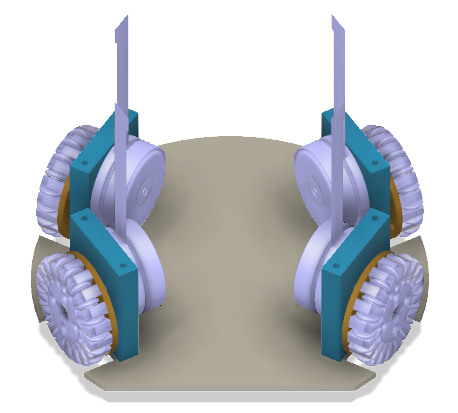
\includegraphics[scale=0.6]{Images/Base_Motores.jpeg}
    \caption{General view of motor distribution. }
    \label{fig:BM}
\end{figure}

\begin{figure}[H]
    \centering
    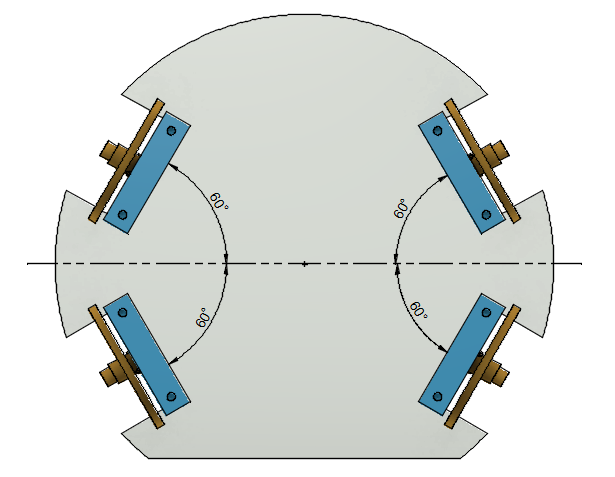
\includegraphics[scale=0.5]{Images/Base_Motores_3.jpeg}
    \caption{Top view motor distribution. }
    \label{fig:BM3}
\end{figure}

With these changes, more space is achieved inside and a symmetric distribution of movement. Likewise it is possible to reduce the necessary height with respect to the model presented last year  \cite{ais2018tdp}.

\subsection{Wheel}

Each block of wheels is redesigned in order to reduce space and standardize the model. For this the diameter of the wheel is reduced, an internal gear is designed and fitted. A model of the assembled system can be seen in the Figure \ref{fig:Wheel1}.

\begin{figure}[H]
    \centering
    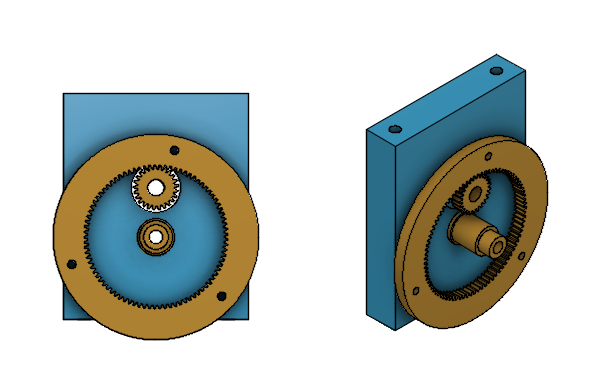
\includegraphics[scale=0.6]{Images/Engranaje.jpeg}
    \caption{Front and general view of gear system. }
    \label{fig:Wheel1}
\end{figure}

The gear set is designed with a gear ratio of 1/3, module 0.4 and 12 mm center distance producing gears of 60 and 20 teeth. With this we can build a symmetrical movement system, where each block can be used in any position as seen in the figure \ref{fig:BM3}.

Finally, to ensure a compact construction, the diameter of the wheel is reduced to 50 mm as seen in the figure \ref{fig:Wheel2} and to produce a more continuous and smooth movement the number of small wheels is increased, from 16 to 18.

\begin{figure}[h]
    \centering
    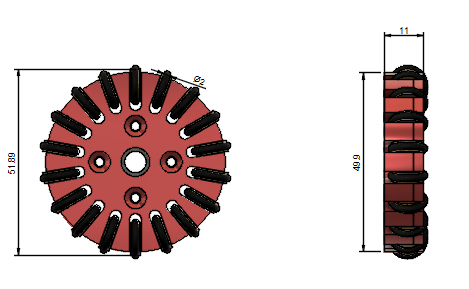
\includegraphics[scale=0.6]{Images/Wheel.jpeg}
    \caption{Front and lateral view of assembled wheel. }
    \label{fig:Wheel2}
\end{figure}

\subsection{Dribbler}

During the game the ball reaches high speeds, that is why you must add a system that cushions the impact of a pass or a shot in order to maneuver or manipulate the ball properly. A correction is proposed in figure \ref{fig:dribbler} to the system mentioned in \cite{ais2018tdp} that adds a degree of freedom that together with a damping sponge allows to solve this problem.

\begin{figure}[h]
    \centering
    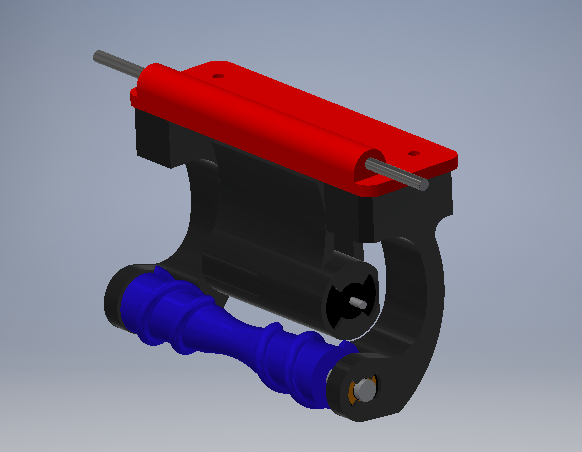
\includegraphics[scale=0.6]{Images/Dribbler.jpeg}
    \caption{General view of assembled dribbler. }
    \label{fig:dribbler}
\end{figure}

\subsection{Motors}
\label{Encoder}

For this year, the aim is to improve the speed control both in motion engines and in the dribbler, that is why the engines are updated to versions with integrated encoder Maxon EC45 flat 50W \cite{MaxonEC45} and Maxon EC-max 22 \cite{MaxonECmax}. For more explanation in use, review the section \ref{ssec:MotionControl}



%%%%%%%%%%%%%%%%%%%%%%%%%%%%%%%%%%%%%%%%%%%%%%%%%%%%%%%%%%%%%%%%%%%%%%%%%%%%%%%%%%%%%%%%%%%%%%%
%                                 Software                                                    %
%%%%%%%%%%%%%%%%%%%%%%%%%%%%%%%%%%%%%%%%%%%%%%%%%%%%%%%%%%%%%%%%%%%%%%%%%%%%%%%%%%%%%%%%%%%%%%%
\section{Software}
The diagram of the figure \ref{fig:gDiagram} shows the general behavior of our system, which after receiving the data delivered by the camera, the referee and the sensors integrated in our robots, begins to evaluate the state of the game in order to take the better decision based on the data previously collected. Then our path planning algorithm is responsible for choosing the path to follow for each robot so that they can achieve the move avoiding any obstacle.

\begin{figure}[H]
    \centering
    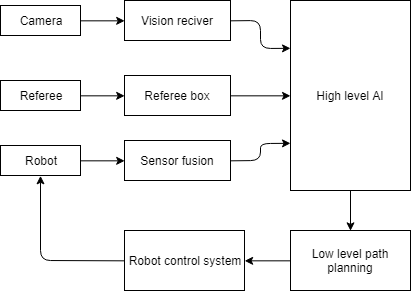
\includegraphics[scale=0.5]{gDiagram.png}
    \caption{General diagram of the system}
    \label{fig:gDiagram}
\end{figure}

We are implementing a client software to host the AI, it gets the information broadcasted by ssl-vision or grSim through Protobuf, filters, process, and sends the data to the communication base station connected by USB (described in section \textit{Communication}). A GUI (figure \ref{fig:GUI}) done in QT allows the user to see what is happening in the field, as well as to monitor plays and formations. The interface contains options for controlling a robot with the keyboard, buttons to control the Referee, monitor the scoreboard, etc.

\begin{figure}[h]
    \centering
    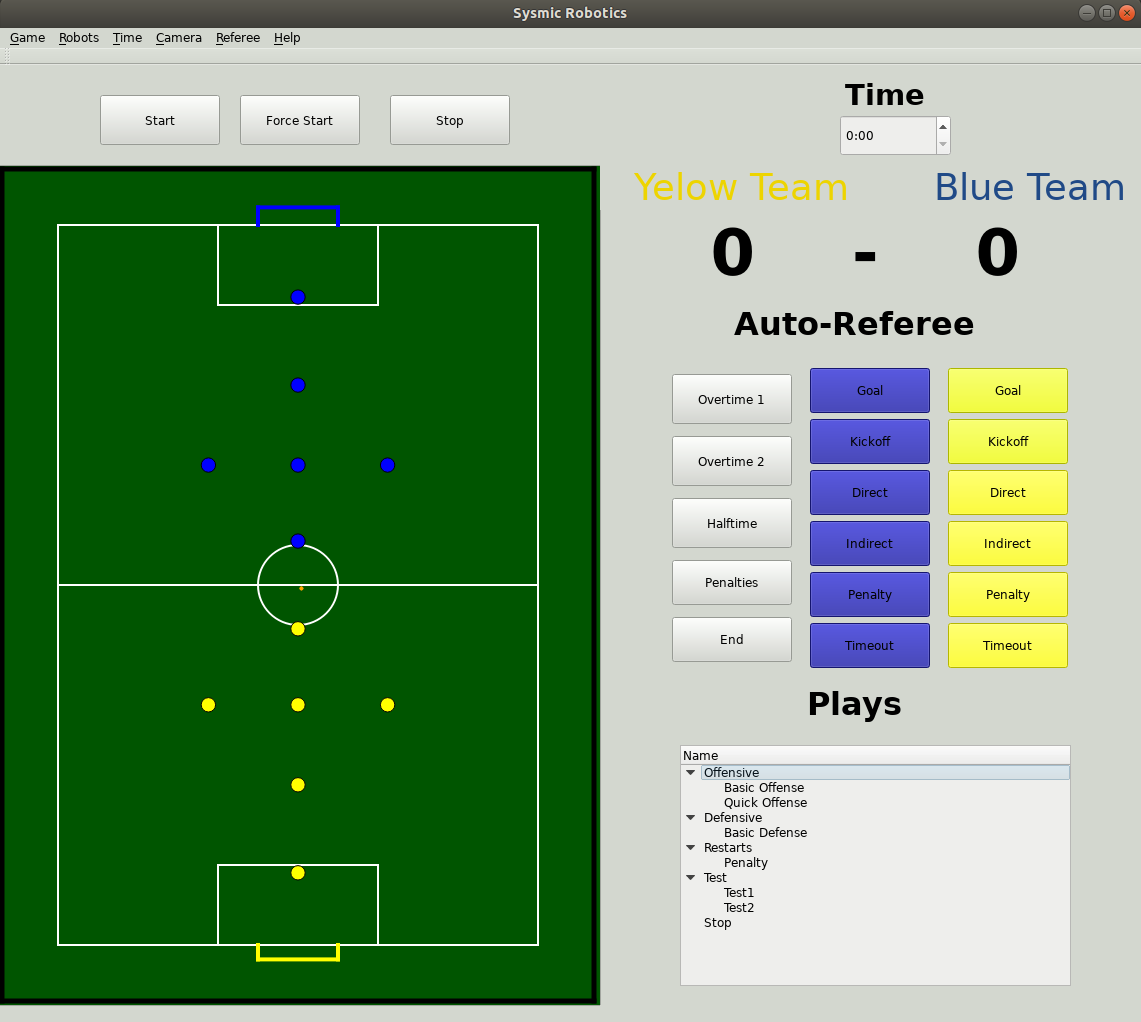
\includegraphics[scale=0.4]{GUI_F.png}
    \caption{GUI screenshot}
    \label{fig:GUI}
\end{figure}

It must be noted that this client is under construction and that we guided ourselves by the software shared by RoboJackets \cite{robojackets}. 

%%%%%%%%%%%%%%%%%%%%%%%%%%%%%%%%%%%%%%%%%%%%%%%%%%%%%%%%%%%%%%%%%%%%%%%%%%%%%%%%%%%%%%%%%%%%%%%
%                                   Sensors                                                   %
%%%%%%%%%%%%%%%%%%%%%%%%%%%%%%%%%%%%%%%%%%%%%%%%%%%%%%%%%%%%%%%%%%%%%%%%%%%%%%%%%%%%%%%%%%%%%%%
\subsection{Sensor Integration}
In the new model we integrate different kind of sensors, meaning that the robots will no longer be a peripheral to take active part in the designed AI system. The goal is to get a better estimate of the game state to enable better decision making at software level improving the game strategy, as well as at hardware level enabling a better control of the robots. Specifically we add encoders, accelerometer, gyroscope and proximity sensors.

Since the omnidirectional robots represent a nonlinear system we implement an Extended Kalman Filter  to make use of the information coming from the different kind of sensors. The main function of this algorithm is to reduce the error coming from the uncertainty present in the environment and in sensor measurement.

The encoders, accelerometer and gyroscope let us get a quicker estimate of the robot pose and velocity, since these components have a high measurement rate. However the downside of this approach is that the error propagates with the robot movement because it is relative to the robot local pose. To correct this increasing error we use the slower measurements coming from the camera taking advantage of its absolute error (since it does not depend of the robot pose and, thus, it does not propagate with it).    

Another important aspect relates to track the ball's position where we mainly use the camera information, but because of the fast nature of the game, there are significant periods of time where the robot does not know where the ball is. For that reason we implement proximity sensors to aid in the ball location when precision is needed.  

%%%%%%%%%%%%%%%%%%%%%%%%%%%%%%%%%%%%%%%%%%%%%%%%%%%%%%%%%%%%%%%%%%%%%%%%%%%%%%%%%%%%%%%%%%%%%%%
%                             High Level AI                                                   %
%%%%%%%%%%%%%%%%%%%%%%%%%%%%%%%%%%%%%%%%%%%%%%%%%%%%%%%%%%%%%%%%%%%%%%%%%%%%%%%%%%%%%%%%%%%%%%%
\subsection{High Level AI}

The high level artificial intelligence maintains the structure described in \cite{ais2018tdp} and is based on the software done by RoboJackets \cite{robojackets}, which is the following: it begins with the scene rater which evaluates and synthesizes the current state of the game, then the play chooser begins making use of the information and thus choose the most optimal play according to the evaluation done by the algorithm. Finally, the role assigner is responsible for selecting which robot meets the requirements set by the play.

\begin{figure}[h]
    \centering
    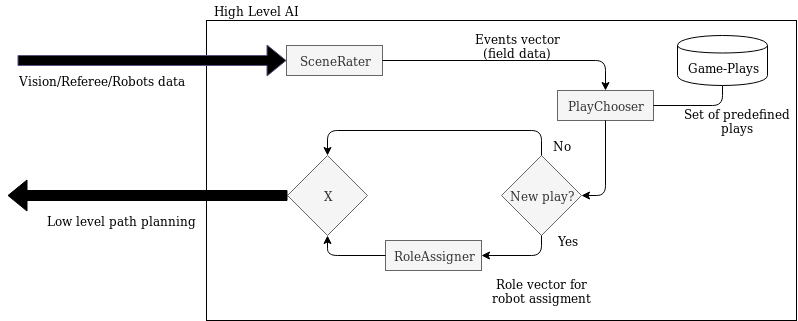
\includegraphics[scale=0.4]{aiDiagram.png}
    \caption{High level AI Diagram}
    \label{fig:ai}
\end{figure}


%%%%%%%%%%%%%%%%%%%%%%%%%%%%%%%%%%%%%%%%%%%%%%%%%%%%%%%%%%%%%%%%%%%%%%%%%%%%%%%%%%%%%%%%%%%%%%%
%                           Low Level path planning                                           %
%%%%%%%%%%%%%%%%%%%%%%%%%%%%%%%%%%%%%%%%%%%%%%%%%%%%%%%%%%%%%%%%%%%%%%%%%%%%%%%%%%%%%%%%%%%%%%%
\subsection{Low Level Path Planning}
The algorithm that is currently being tested is RRT* \cite{RRT}, which works similarly to RRT (algorithm already described in \cite{ais2018tdp}), the Algorithm \ref{rrt2} (lines 8-14) RRT* also extends the new vertex to the vertices in $X_{near}$ in order to "rewire" the vertices that can be accessed through $X_{new}$ with smaller cost.

\begin{algorithm}[h]
\caption{Rapidly Exploring Random Trees Star}
\begin{algorithmic}[1]
    \Procedure{BUILD-RTT($x_{init}$)}{}
        \State $T.init$ 
        \For{$x_{near} \epsilon X_{near}$}
            \State $x_{rand} \gets \text{RandomState()}$
            \State $\text{EXTEND}(T,x_{rand})$
        \vspace{0.1em}
        \EndFor
        \For{$x_{near} \epsilon X_{near}$}
            \State $\text{REWIRE}(T,x_{rand},x_{near})$
        \vspace{0.1em}
        \EndFor
        \Return $T$
    \EndProcedure
\end{algorithmic}
\label{rrt}
\end{algorithm}

\begin{algorithm}[h]
%\caption{}\label{euclid}
\caption{procedures involved on RRT*}
\begin{algorithmic}[1]
    \Procedure{EXTEND($T$,$x$)}{}
        \State $x_{near} \gets \text{NEAREST-NEIGHTBOR()}$
        \If{NEW-STATE($x_{goal},x_{near},x_{new},u_{new}$)}
            \State $T.\text{add-vertex}(x_{new})$
            \State $T.\text{add-edge}(x_{near},x_{new},u_{new})$
            \If{$x_{new} = x$}
                \Return $Reached$
            \Else{}
                \Return $Advanced$
            \EndIf
        \vspace{0.4em}
        \EndIf
        \Return $Trapped$
    \EndProcedure
    \Procedure{REWIRE($T$,$x$)}{}
        \State $x_{near} \gets \text{NEAREST-NEIGHTBOR()}$
        \State $x_{parent} \gets \text{PARENT} (x_{near})$
        
        \If{Cost($x_{new},x_{near},u_{new}$) $<$ Cost($x_{parent},x_{near}$)}
            \State $T.\text{remove-edge}(x_{near},x_{parent},u_{new})$
            \State $T.\text{add-edge}(x_{parent},x_{new},u_{new})$
        \EndIf
        \Return Rewired
    \EndProcedure
\end{algorithmic}
\label{rrt2}
\end{algorithm}


%%%%%%%%%%%%%%%%%%%%%%%%%%%%%%%%%%%%%%%%%%%%%%%%%%%%%%%%%%%%%%%%%%%%%%%%%%%%%%%%%%%%%%%%%%%%%%%
%                               HARDWARE
%
%%%%%%%%%%%%%%%%%%%%%%%%%%%%%%%%%%%%%%%%%%%%%%%%%%%%%%%%%%%%%%%%%%%%%%%%%%%%%%%%%%%%%%%%%%%%%%
\section{Hardware}
\subsection{$\mu$Controller}
\label{sec:hw_micro}
This year, the hardware that controls the robot has been modified in mainly to give more functionalities to the robot, being more competitive than its predecessor. In this way, the 5 PIC32MX440F256H used in its previous version (one as a control unit and the remaining 4 for motor control as shown in Figure \ref{fig:hw_old}) was replaced by an STM32F767BIT6 of ST electronics, which has among its features:  Cortex®-M7 32-bit core Arm®, up to 216MHz, 462 DMIPS, 2Mbytes of flash memory, graphics drivers, 4 I2C, 6 SPI and 168 GPIO as described in \cite{STdatasheet}. These capabilities, together with their ease of use, make this new microcontroller a necessary component for this new version.

In addition, an accelerometer and a gyroscope were added to the board (both described in section \ref{sec:hw_accel}) in order to improve robot on-board odometry. The old communication of the robots using APC220 with the central PC was modified to use NRF24, which significantly increases the transmission bitrate. This means better reaction time of robots when they receive instructions from central PC.  For the detection of the ball, the VL6180X sensor is used, which is a TOF sensor with a range of 5mm to 100mm distance.

\begin{figure}[H]
    \centering
    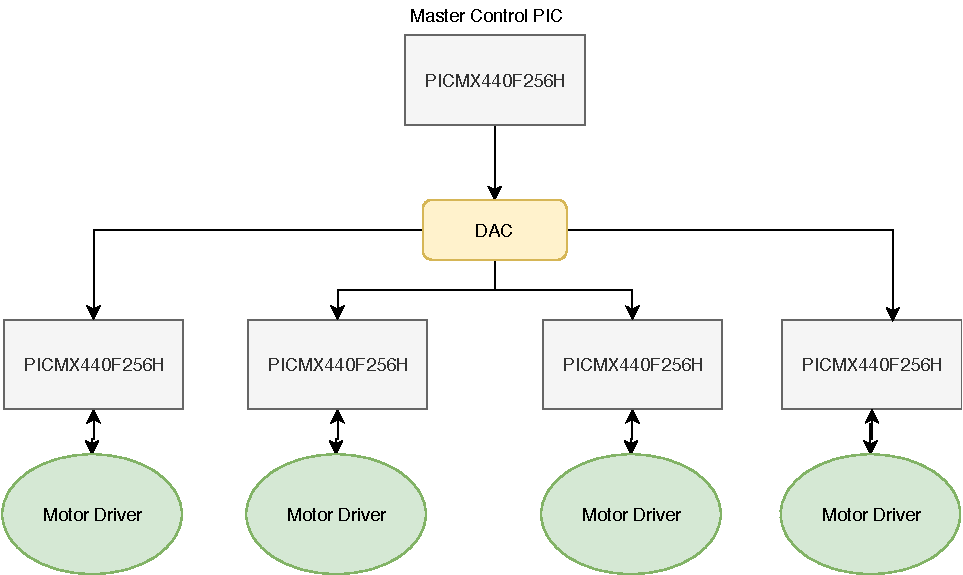
\includegraphics[width=0.9\textwidth]{Images/HardwareOLD.pdf}
    \caption{Previous Hardware Architecture}
    \label{fig:hw_old}
\end{figure}

The new hardware architecture (Figure \ref{fig:hw_new})
makes the control system of motors and, as is previously stated, the robot odometry more efficient given that this features are only dependent of one component (STM32 $\mu$controller), and the failure of one module is independent of any communication issues in another part of the board.

\begin{figure}[H]
    \centering
    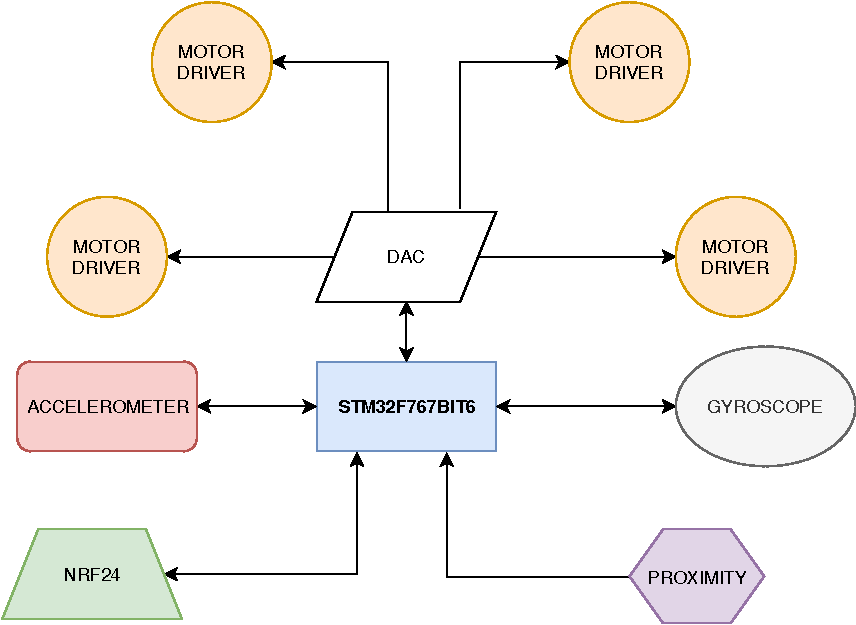
\includegraphics[width=0.8\textwidth]{Images/HardwareNew.pdf}
    \caption{Actual Hardware Architecture}
    \label{fig:hw_new}
\end{figure}

\subsection{Accelerometer and Gyroscope} \label{sec:hw_accel}
\justify This two new components are low power consumption,the Accelerometer (ADXL312ACPZ) has a resolution measurement up to $\pm 12g$ and it is connected using SPI to STM $\mu$controller because of this high speed bit rate \cite{adxl312_datasheet}. The Gyroscope (FXAS21002CQR1) has a resolution up to $\pm 0.0625^\circ$ configurable and an output data rate up to 200Hz\cite{gyro_datasheet}. Both components are connected to an individual SPI bus of STM $\mu$controller, this make more easy to debug if any problem occurs.

\subsection{Proximity}
Previous version of Sysmic robots hadn't a proximity sensor, that make the playability and behaviour of robots extremely inefficient because they were completely dependent of main PC server's processing speed and they were not capable to detect when a kick action was correct or not. In this version we add a proximity sensor (VL6180X of ST electronics) which has a measurement range of 5mm to 100mm \cite{proximity_data} which make this new component a great tool to detect presence of the ball and add precision to robot gestures and plays, also with this new feature robots are capable to do plays and take decisions independent of main PC server.

%%%%%%%%%%%%%%%%%%%%%%%%%%%%%%%%%%%%%%%%%%%%%%%%%%%%%%%%%%%%%%%%%%%%%%%%%%%%%%%%%%%%%%%%%%%%%%%
%                                 Main PCB                                                    %
%%%%%%%%%%%%%%%%%%%%%%%%%%%%%%%%%%%%%%%%%%%%%%%%%%%%%%%%%%%%%%%%%%%%%%%%%%%%%%%%%%%%%%%%%%%%%%%
\subsection{Main Board}
In addition to what was said in in \ref{sec:hw_micro} the new features of STM32F767BIT6 allow us to increase performance of robots, and the new components added in this version allow us to improve odometry and reaction time of the robots. The previous version of Main Board has a serious problem of noise in the board, that was because it does not separate power ground of control ground. To reduce the noise and interference in the components the new  board was designed with 4 layers.

\begin{figure}[H]
    \centering
    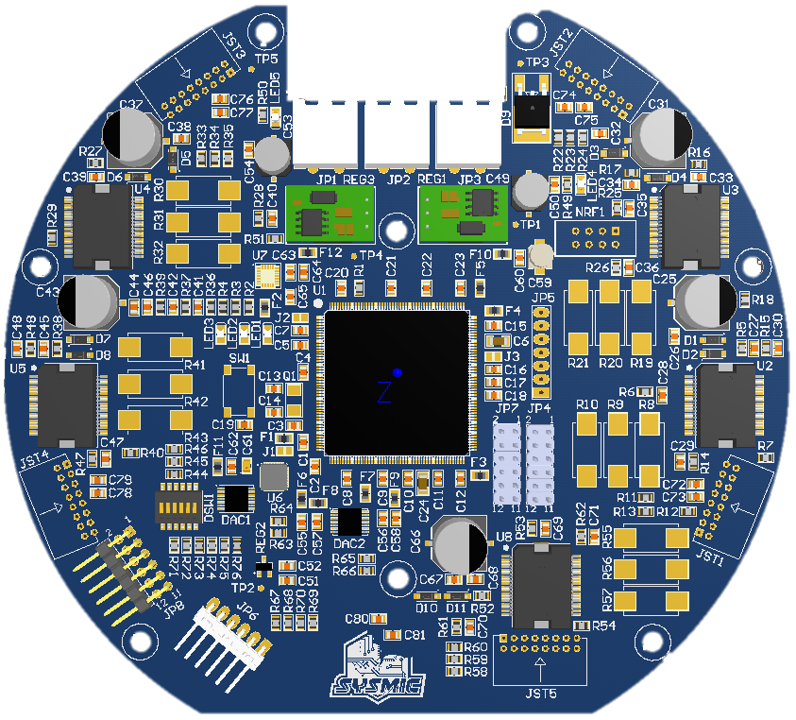
\includegraphics[scale=0.4]{PCB_3D_1.PNG}
    \caption{Main Board}
    \label{fig:main_board}
\end{figure}


%%%%%%%%%%%%%%%%%%%%%%%%%%%%%%%%%%%%%%%%%%%%%%%%%%%%%%%%%%%%%%%%%%%%%%%%%%%%%%%%%%%%%%%%%%%%%%%
%                                 Communication                                                %
%%%%%%%%%%%%%%%%%%%%%%%%%%%%%%%%%%%%%%%%%%%%%%%%%%%%%%%%%%%%%%%%%%%%%%%%%%%%%%%%%%%%%%%%%%%%%%%
\subsection{Communication}
Looking forward to improving the communication system we chose to change our former communication device due its speed capabilities, robustness and scalability. One of the main approaches to this new communication system is to guarantee persistence in the flow of the packets, so an intelligent node is being developed to guarantee no losses.

As described in \cite{ais2018tdp} the communication link between software and robots of former system was composed by APC220 transceivers, which communication strategy involves transparent packet transmission in a UART/TTL interface, whose maximum baudrates were 19200 by air and 57600 once linked to decoder MCU. Due to device capabilities and low data rate transmission, giving feedback from robots to software does not provide reliability so scalability is not possible under this scheme.

Subsequently by running multiple tests on NRF24L01$+$, we choose it as a reliable option and, as seen in SSL category, it is prefered by most teams due his features: $2.4[\text{GHz}]$ band operation, ultra low power operation, up to 2Mbps air data rate and robust packet handling. The communication between the transceiver and software is done by connecting a STM32F401 MCU to the computer of the team by its OTG controller in full speed operation, which allow the MCU to receive packets of data related to motion and actions of the robots on the field at a rate of 12Mbits/s. The NRF24L01$+$ is connected to the MCU by SPI interface that communicates the data sent from software with the transceiver, whose transfer this data to the robots.

In \cite{tigers2018etdp} a communication base station is presented with HMI features included that show the state of each robot and information related to SSL Vision and SSL Refbox. In a similar approach our communication system will store data of the state of the robots on the field, that allow to monitor their status, develop emergency routines and run test tasks on them.


%%%%%%%%%%%%%%%%%%%%%%%%%%%%%%%%%%%%%%%%%%%%%%%%%%%%%%%%%%%%%%%%%%%%%%%%%%%%%%%%%%%%%%%%%%%%%%%
%                                 Kicker                                                      %
%%%%%%%%%%%%%%%%%%%%%%%%%%%%%%%%%%%%%%%%%%%%%%%%%%%%%%%%%%%%%%%%%%%%%%%%%%%%%%%%%%%%%%%%%%%%%%%
\subsection{Kicker}
%\RK{descripcion del pateador flyback}[Ruben: si existe una imagen mejor del circuito (vector), hay que actualizarla]

In the former version of our robots, the circuit of the kicking system was a Boost converter as shown in the Figure \ref{fig:old_boost}. This converter raises the voltage from the battery to 120 [V], but the main disadvantage of the circuit is the charging time, taking about 6 seconds to reach the final value. Given the dynamics and speed of the game, this charging time is excessive.

\begin{figure}[h]
    \centering
    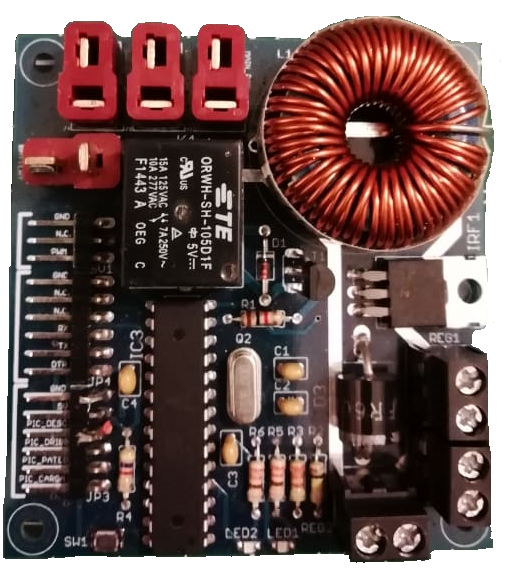
\includegraphics[width=0.5\textwidth]{Images/foto_boost.jpg}
    \caption{Old Boost circuit}
    \label{fig:old_boost}
\end{figure}

This year, the kicking system has been modified and now consists in a flyback circuit as shown in the Figure \ref{fig:kicker}. This circuit uses the Chip LT3751 which is a charger controller with regulation. The flyback circuit implements a turn ratio of 1:10 (primary:secondary) and raises the voltage from 14.8 [V] to 220 [V] on two capacitors of 1200[$\mu$F], each in less than a half second. The main advantage is that the voltage setpoint can be regulated to kick with different intensities.
%\TR{Esta imagen esta repetida en el TDP 2018. Si no hay cambios en el diseño no deberiamos ponerlo.}

\begin{figure}[h]
    \centering
    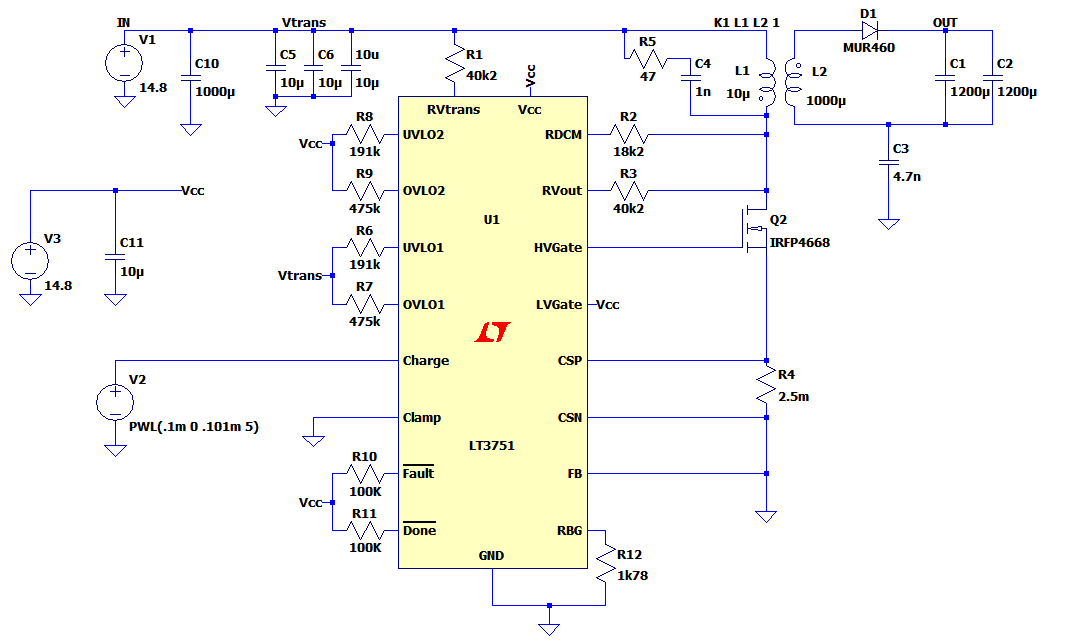
\includegraphics[scale=0.4]{Images/kicker_spice.png}
    \caption{Kicker Circuit}
    \label{fig:kicker}
\end{figure}

%%%%%%%%%%%%%%%%%%%%%%%%%%%%%%%%%%%%%%%%%%%%%%%%%%%%%%%%%%%%%%%%%%%%%%%%%%%%%%%%%%%%%%%%%%%%%%%
%                                 Motor Control                                               %
%%%%%%%%%%%%%%%%%%%%%%%%%%%%%%%%%%%%%%%%%%%%%%%%%%%%%%%%%%%%%%%%%%%%%%%%%%%%%%%%%%%%%%%%%%%%%%%
\subsection{Motor control} \label{ssec:MotionControl}

In order to enhance the motion of the robots, an accurate motor speed control loop is incorporated to the hardware system. The previous design, as described in \cite{ais2018tdp}, does not have encoders to measure the rotational speed in the motors and use the feedback information generated by hall sensors, causing the robot to have erratic movements mostly in low speed movements. Actual design incorporate a MILE Encoder with 2048 CPT by Maxon, increasing measure precision and allowing the discrete controller to increase the sample time significantly.

Speed control in the motors is managed by a PID controller designed in MATLAB by controlling the BLDC motor plant from the data provided by datasheet. The motor used is an EC 45 flat brushless, 50 Watt, with Hall sensors by Maxon. Fig. \ref{fig:pid_schematic} shows the controller block schematic implemented for the motor speed control task, where the gray block representing the closed loop is repeated for each wheel.

\begin{figure}[h]
    \centering
    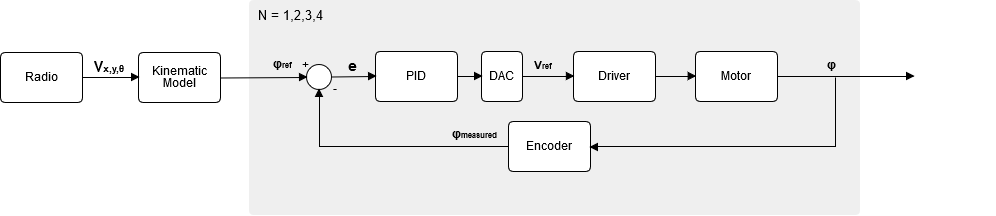
\includegraphics[width=0.9\textwidth]{Images/PID_SCHEMATIC.png}
    \caption{PID Schematic}
    \label{fig:pid_schematic}
\end{figure}

%\PR{https://gifer.com/en/7VE}

%%%%%%%%%%%%%%%%%%%%%%%%%%%%%%%%%%%%%%%%%%%%%%%%%%%%%%%%%%%%%%%%%%%%%%%%%%%%%%%%%%%%%%%%%%%%%%%
%                            Power Source Motor                                               %
%%%%%%%%%%%%%%%%%%%%%%%%%%%%%%%%%%%%%%%%%%%%%%%%%%%%%%%%%%%%%%%%%%%%%%%%%%%%%%%%%%%%%%%%%%%%%%%
\subsection{Power Source Motor}

While in the Robocup 2018, one of the problems we detected in our robot is that the battery was oversized, this caused the space available inside the robot to be reduced. Therefore our team set out to implement a DC-DC boost converter which will allow us to reduce the size of our batteries from a 6s LiPo to a 4s.\\

The LT8711 integrated circuit from Linear Technology is responsible for mosfet switching and the output voltage control. As a design requirement, it is necessary to obtain 24V, as shown in figure \ref{fig:boost1}, and 5A from 14.8V of the 4s LiPo battery. This circuit is designed to drive each of the 4 Maxon EC45 flat 50W motors (see figure \ref{fig:boost}).\\

\begin{figure}[h]
    \centering
    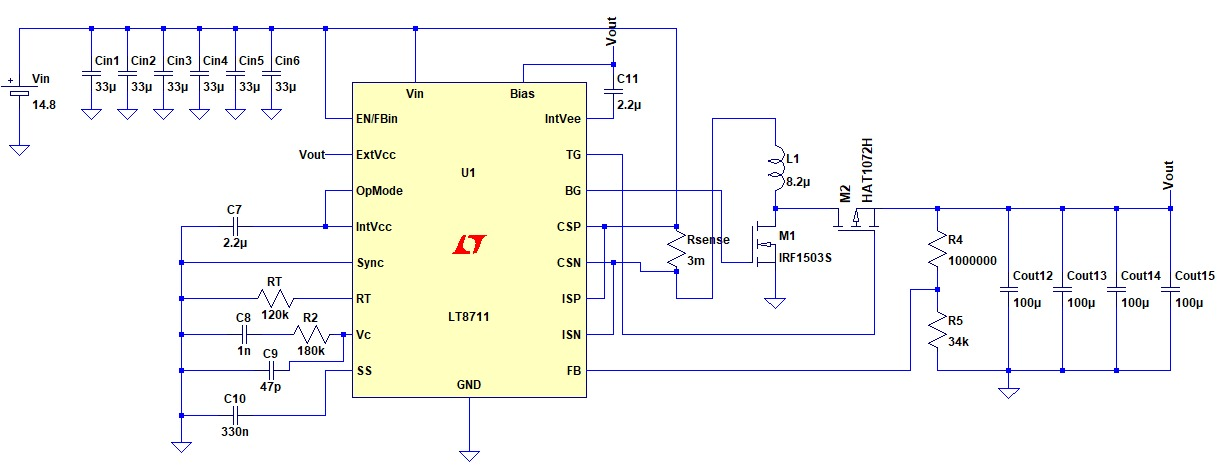
\includegraphics[width=1.1\textwidth]{Images/Power_source_motor.png} 
    \caption{Boost circuit}
    \label{fig:boost}
\end{figure}

Furthermore, this module is responsible of measuring the voltage of each battery cell preventing them from being discharged lower than 3.7V. For this, an Attiny84 will be used, which will alert the main board in case it is discharged. The first version of the circuit is in the figure \ref{fig:boost2}.

\begin{figure}[H]
    \centering
    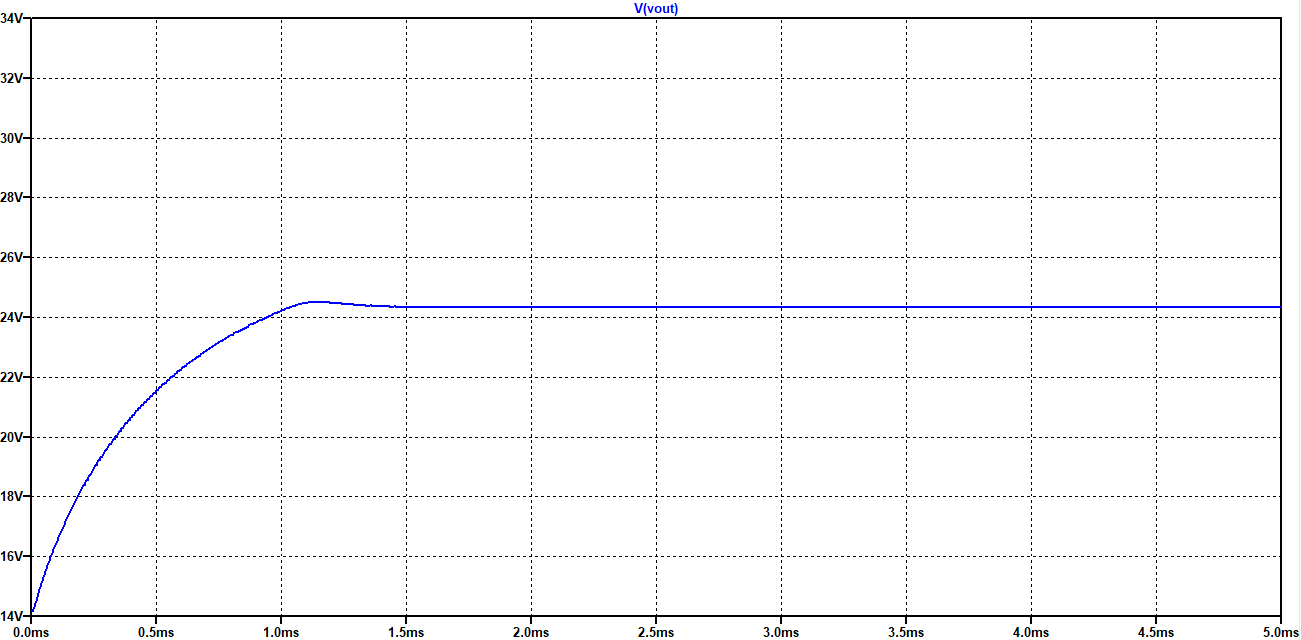
\includegraphics[width= 0.9\linewidth, clip]{Images/Power_source_motor1.png}
    \caption{Boost circuit plot}
    \label{fig:boost1}
\end{figure}

\begin{figure}[H]
    \centering
    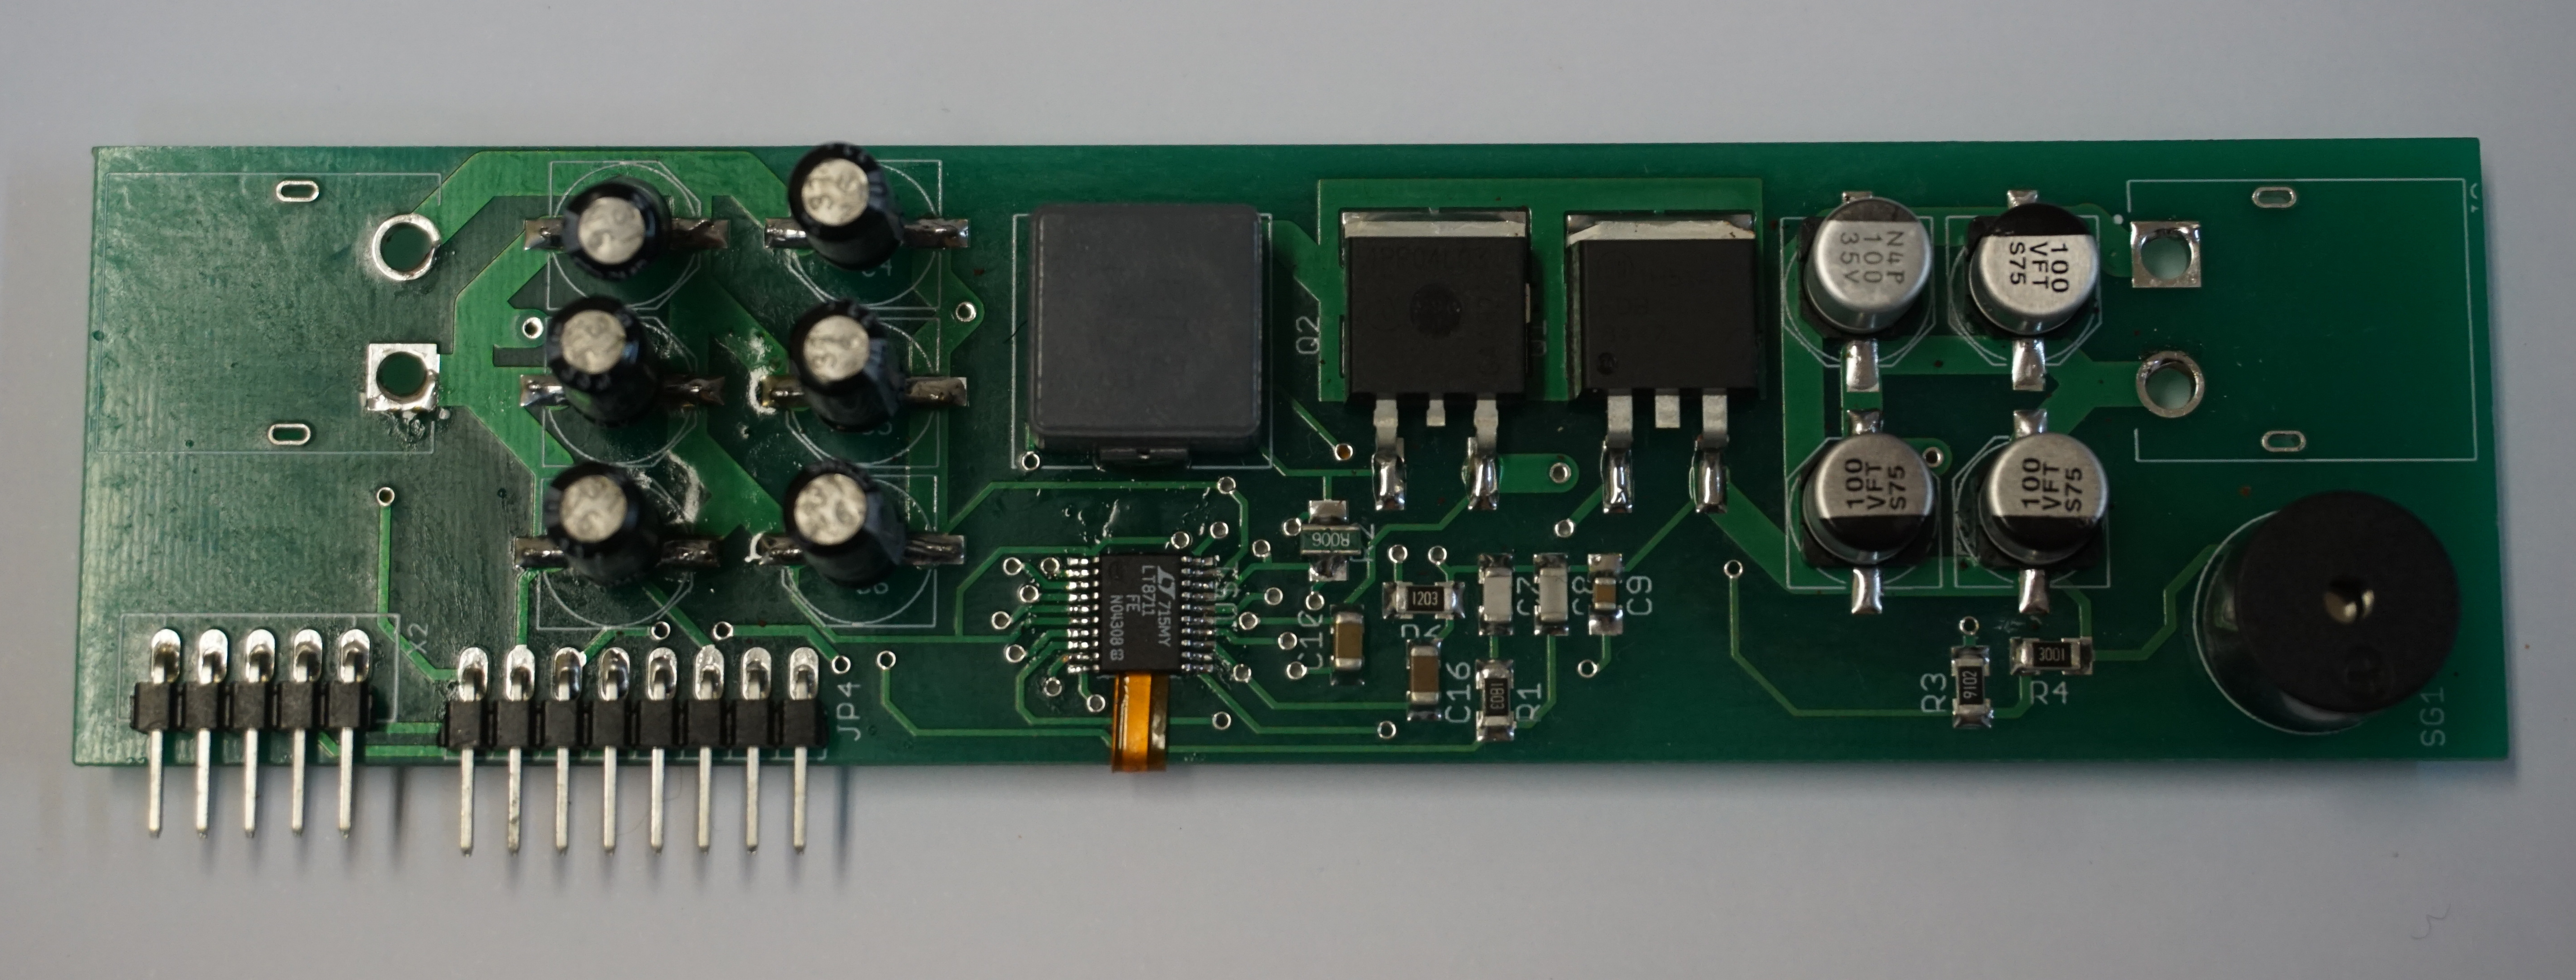
\includegraphics[width= \textwidth, clip]{Images/Power_source_motor2.png}
    \caption{Implemented boost and control voltage level circuit}
    \label{fig:boost2}
\end{figure}

%%%%%%%%%%%%%%%%%%%%%%%%%%%%%%%%%%%%%%%%%%%%%%%%%%%%%%%%%%%%%%%%%%%%%%%%%%%%%%%%%%%%%%%%%%%%%%%
%                                 Bibliografy                                                 %
%%%%%%%%%%%%%%%%%%%%%%%%%%%%%%%%%%%%%%%%%%%%%%%%%%%%%%%%%%%%%%%%%%%%%%%%%%%%%%%%%%%%%%%%%%%%%%%
\bibliographystyle{plain}
{
    \renewcommand{\clearpage}{} 
    \bibliography{biblio.bib}
}



%%%%%%%%%%%%%%%%%%%%%%%%%%%%%%%%%%%%%%%%%%%%%%%%%%%%%%%%%%%%%%%%%%%%%%%%%%%%%%%%%%%%%%%%%%%%%%%
%                             Acknowledgments                                                 %
%%%%%%%%%%%%%%%%%%%%%%%%%%%%%%%%%%%%%%%%%%%%%%%%%%%%%%%%%%%%%%%%%%%%%%%%%%%%%%%%%%%%%%%%%%%%%%%
\section*{Acknowledgments}

Sysmic Robotics would like to acknowledge the previous team members that helped us to get here and to all the people that support and help us in any way. We could not have made it alone.

% that's all folks
\end{document}